\subsection{Level2.3: $y=-x*sin(x)$ について}

% 問題意識: 効率良く最適解(目的物)を探し出すにはどうしたら良いだろうか?
% 
% Level2.xでは、解空間が連続値であり、目的関数や制約条件が数式として定義されているという前提で「最適値を効率良く求める」ことについて理解を深めていこう。

% レポートに含める項目
% プログラムソース(スクリプトを含む)。
% レポート内には変更個所のみを記載した上で、ソース全体はアップロード提出すること。
% 
% 観察意図と観察方法(実験計画)。コメント: どうやれば最適性or効率性を検討できるだろうか?
% 実行結果。
% 無駄に全てを示す必要はなく、第三者が読んでも理解できる程度に、必要十分に示すこと。
% 
% 考察。
% 特に「学習係数が探索挙動に及ぼす影響」として「得られた解の質」と「効率性」について考察すること。 (どう検証したら良いだろうか?)
% 
% 必要に応じて適切な図表を作成し、理解しやすい考察となるようにすること。


% 今回は「最適性」と「効率性」という視点で考察できるように実験計画を練ってみてください。
\subsubsection{プログラムソース(変更部分)}
Level2.3ではsteepest\_decent.cのf関数とpd\_x関数を一部以下のように変更した.
\begin{itembox}[c]{f(x,y)関数の変更点}
    {\small
    \begin{verbatim}
    double f(double x, double y) {
        double z;

        /** 以下の式を編集して完成させよ(1) **/
        //z = x;
        z = -x * sin(x);

        return( z );
    }
    \end{verbatim}
}
\end{itembox}

\begin{itembox}[c]{pd\_x(x,y)関数の変更点}
    {\small
    \begin{verbatim}
    double pd_x(double x, double y) {
        double z_dx;

        /** 以下の式を編集して完成させよ(2-1) **/
        //z_dx = 1;
        z_dx = -sin(x) - x*cos(x);

        return( z_dx );
    }
\end{verbatim}
}
\end{itembox}

\subsubsection{観察意図と観察方法(実験計画)}
最急降下法は,$y=x^2$のような「極小値=関数全体の最小値」となる
関数に対しては非常に有効なアルゴリズムである.
しかし,今回の$y=-xsin(x)$のように極小値が複数ある場合は,
探索開始地点から最寄りの極小値に収束しようとする.
これは必ずしも関数の最小値だとは限らない.
そのため,複数の初期値を与えて実行し,それぞれの収束したときの
$y$の値の中から最も小さいものを選択すれば,それが関数の最小値
となるだろうと考えた. \\
 run\_ave.shをベースに試行回数10回分の結果の中から$y$の最小値を
抜き出すスクリプト(ソースコード\ref{alter})を作成した.
また学習係数$\alpha$を変えることにより,どのようにstep数が
変動するかを観察する.

\lstinputlisting[caption=$y$の最小値を求めるプログラム,label=alter]{./figs/alter_run_ave.sh}


\subsubsection{実行結果}
% alter_hogehoge.shとrunなんちゃら,trans_step,trans_x_も
% やる
%
今回試した学習係数$\alpha$は$0.075, 0.2$の2つである.
まず,ソースコード\ref{alter}を実行した結果を示す.

\begin{itembox}[c]{$\alpha=0.075$の時に求まった$-xsin(x)$の最小値}
    {\small
        \begin{verbatim}
        /Users/e135761/search/steep/steepestsearch% ./alter_run_ave.sh
        FINISH 3 step 72 x and y were not updated.
        FINISH 3 step 17 x and y were not updated.
        FINISH 3 step 59 x and y were not updated.
        FINISH 3 step 19 x and y were not updated.
        FINISH 3 step 67 x and y were not updated.
        FINISH 3 step 23 x and y were not updated.
        FINISH 3 step 24 x and y were not updated.
        FINISH 3 step 68 x and y were not updated.
        FINISH 3 step 19 x and y were not updated.
        FINISH 3 step 61 x and y were not updated.
        -7.9167273716
        /Users/e135761/search/steep/steepestsearch%
        \end{verbatim}
    }
\end{itembox}

\begin{itembox}[c]{$\alpha=0.2$の時に求まった$-xsin(x)$の最小値}
    {\small
        \begin{verbatim}
        /Users/e135761/search/steep/steepestsearch% ./alter_run_ave.sh
        FINISH 3 step 24 x and y were not updated.
        FINISH 3 step 36 x and y were not updated.
        FINISH 3 step 19 x and y were not updated.
        FINISH 3 step 35 x and y were not updated.
        FINISH 3 step 22 x and y were not updated.
        FINISH 3 step 38 x and y were not updated.
        FINISH 3 step 36 x and y were not updated.
        FINISH 3 step 22 x and y were not updated.
        FINISH 3 step 34 x and y were not updated.
        FINISH 3 step 20 x and y were not updated.
        -7.9167273716
        /Users/e135761/search/steep/steepestsearch%
        \end{verbatim}
    }
\end{itembox}
特に$\alpha$による最小値の違いは見られなかった.
ここで,得られた最小値がどれほどの精度なのかを知るため,方程式の解の近似値を求める手法であるニュートン法\cite{newton}(ソースコード\ref{newton})で同様のことを行った.
ここでいう方程式は,$y=-xsin(x)$の導関数が0になる式,すなわち$y'=-sin(x) - xcos(x)=0$のことである.
この方程式を解くことで関数が最小値をとるときの$x$を求めることができる.

\lstinputlisting[caption=ニュートン法による最小値算出,label=newton]{./figs/Newton.scala}

\begin{itembox}[c]{ニュートン法による最小値の算出結果}
    {\small
        \begin{verbatim}
        /Users/e135761/scala% scala Newton
        x is 7.978665712413194
        the minimum value is -7.916727371587782
        /Users/e135761/scala%
        \end{verbatim}
    }
\end{itembox}

この実行結果は上記のようになり,最急降下法で得られた最小値はほぼ正確なものだと言える. \\
 次に,run\_ave.shを用いて$\alpha$が0.075と0.2のときのそれぞれの
平均step数を調べたところ,$\alpha=0.075$のとき平均step数は
41.90で,$\alpha=0.2$のときのそれは27.60であった.

% \begin{itembox}[c]{}
%     {\small
%         \begin{verbatim}
%         \end{verbatim}
%     }
% \end{itembox}

\subsubsection{考察}

実験結果より,2つの学習係数$\alpha$間で最小値の精度に違いは見られず,
かつ,ニュートン法との比較でそれは正確なものだと判断できるため,
得られた解は解の質として好ましいものである.
効率性に関しては,少ないstep数で最小値に収束している
$\alpha=0.2$の方が効率的であることが分かる
(図\ref{fig:sim-6000-0.2},図\ref{fig:sim-6000-0.075}).
学習係数$\alpha$にあまりに小さい値をとると,解を求めるファクターとしての最適性は十分に有するものの,効率性に欠けるという欠点が
生じる.
反対に大きすぎる数値を学習係数に設定すると,定義域を外れたり,
指定した探索回数内で終了しない原因になる.
したがって学習係数$\alpha$には0.2付近の値を設定するのがよい.


\begin{minipage}{0.5\hsize}
    \begin{figure}[H]
        \begin{center}
            \includegraphics[scale=0.25]{./figs/sim-6000-0_2.eps}
            \caption{$\alpha=0.2$のときの目的関数推移図}
            \label{fig:sim-6000-0.2}
        \end{center}
    \end{figure}
\end{minipage}
\begin{minipage}{0.4\hsize}
    \begin{figure}[H]
        \begin{center}
            \includegraphics[scale=0.25]{./figs/sim-6000-0_075.eps}
            \caption{$\alpha=0.075$のときの目的関数推移図}
            \label{fig:sim-6000-0.075}
        \end{center}
    \end{figure}
\end{minipage}
